\documentclass[journal]{IEEEtran}
\usepackage{graphicx}
\graphicspath{ {./images/} }
\usepackage{booktabs} % for much better looking tables
\usepackage{array} % for better arrays (eg matrices) in maths
\usepackage{paralist} % very flexible & customisable lists (eg. enumerate/itemize, etc.)
\usepackage{verbatim} % adds environment for commenting out blocks of text & for better verbatim
\usepackage{subfig} % make it possible to include more than one captioned figure/table in a single float
\bibliographystyle{IEEEtran}
\bibliography{IEEEabrv,bib.bib}
\title{Analyzing the ACM Citation Network}
\author{Genevieve Peters\\{Big Data Analytics\\University of Illinois Springfield}}

\begin{document}
\maketitle
\section{Introduction} 
The Association for Computing Machinery (ACM) publishes peer reviewed journal articles focused on computer science research \cite{acm}. Tang et al \cite{tang} prepared a dataset consisting of over 2 million articles for the purpose of analyzing the ACM citation network. In this paper, we explore article properties, graph the indegree distribution, rank articles, and quantify clustering. Incremental steps are explained on a small contrived network. The program, written in Scala, uses Spark SQL \cite{sparksql}, Spark GraphX library \cite{graphx}, and Jupyter Notebook.
\section{Methodology} 
The text file was loaded into Spark and its contents were reviewed. The database \cite{tang} is constructed of records, each representing a single article and its metadata is prefixed for easy data extraction. Null records and papers with less than 1 reference were filtered out.\\
\begin{center}
\begin{tabular}{@{}ll}
\textbf{\#*}		& paperTitle \\
\textbf{\#@}	& Authors \\
\textbf{\#t}		& Year \\
\textbf{\#c}		& publication venue \\
\textbf{\#index}	& index id of this paper \\
\textbf{\#\%}	& ids of references of this paper \\
\textbf{\#!}		& Abstract \\\\
\end{tabular}
\end{center}

The articles used in the sample network were taken from the ACM dataset. References were modified to create a small complete graph. There are 6 articles and 11 links between them. The record for one of the articles is shown below.\\\\
\small \#*A Description of the Camellia Encryption Algorithm\\
\#@M. Matsui, J. Nakajima, S. Moriai\\
\#t2004\\
\#cA Description of the Camellia Encryption Algorithm\\
\#index5590e1440cf2baaad9717837\\
\#!This document describes the Camellia encryption algorithm. Camellia is a block cipher with 128-bit block size and 128-, 192-, and 256-bit keys. The algorithm description is presented together with key scheduling part and data randomizing part.\\
\#\%5590dd700cf25001c36ef821\\
\#\%5590e1200cf237666fc297fe
\normalsize
\subsection{Data Extraction}
Useful data (title, index, references) were extracted from each record and stored in an RDD.\\\\
\begin{center}
\small 
(5590e1440cf2baaad9717837, A Description of the Camellia Encryption Algorithm 5590dd700cf25001c36ef821   5590e1200cf237666fc297fe)
\normalsize
\end{center}
Records with more than 1 reference were flattened to isolate each link. Title was removed temporarily until needed during the paper ranking stage.\\\\
(5590e1440cf2baaad9717837, 5590dd700cf25001c36ef821)\\
(5590e1440cf2baaad9717837, 5590e1200cf237666fc297fe)\\\\
To improve performance and ease analysis, the index strings were assigned a unique id. The 11 links are as follows.\\
\begin{center}
\begin{tabular}{ c c c c }
(0, 2)   & (0, 4)   & (0, 3)  & (1, 3)\\
(2, 5)   & (2, 4)  & (3, 4)   & (3, 0)\\
(4, 1)  & (5, 2)   &  (5, 0)\\\\
\end{tabular}
\end{center}
The RDD is then converted to a Graph as shown in Figure 1.
\begin{figure}[h!]
\begin{center}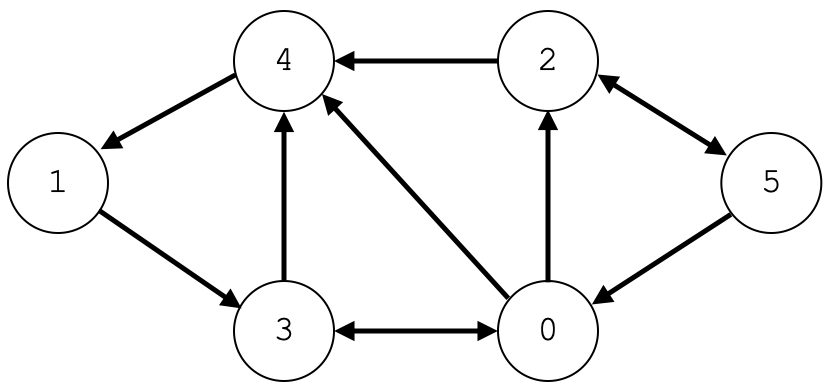
\includegraphics[scale=0.2]{1.png}\end{center}
\caption{The sample dataset in graph form. Articles are shown as circles with their id. Links are shown as directed arrows.}
\end{figure}
\subsection{Degrees}
The degree of an article is the number of links connected to it. The indegree is the number of articles that cite it. The outdegree is the number of articles it references. Since the data is in Graph form, there are 3 functions (.degrees, .inDegrees, .outDegrees) that easily generate these values as shown in Figure 2.\\\\
The indegree distribution of a graph measures the proportion of articles that have a specific indegree. In this sample dataset, there are 3 unique values for indegree (1, 2, 3) as shown in blue on Figure 2. The distribution can be represented on a graph and analyzed. The full ACM dataset, for instance, showed that there were substantially more articles with fewer indegrees. For this sample dataset, the distribution is too small to really gather any valuable information from it.\\
\begin{figure}[h!]
\begin{center}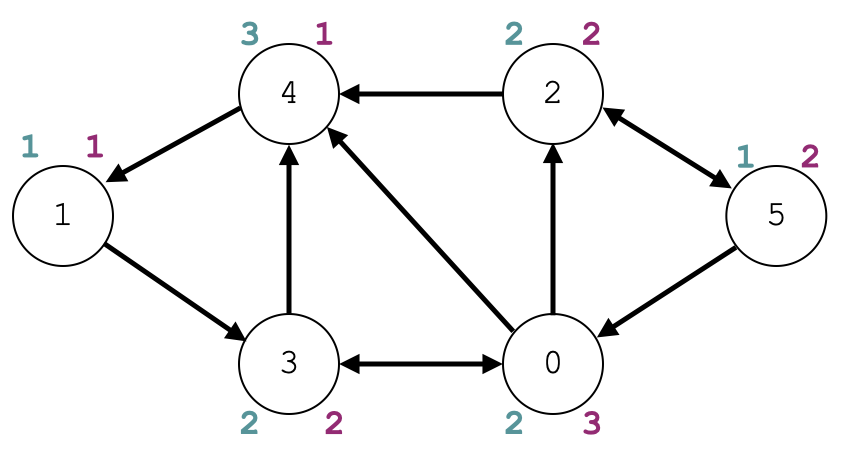
\includegraphics[scale=0.2]{2.png}\end{center}
\caption{The degrees of each article in the graph. Indegrees are represented in blue. Outdegrees are represented in purple. Degrees would simply be the sum of the two.}
\end{figure}
\subsection{In-Weight}
For conciseness, \emph{node} is equivalent to \emph{article}, \emph{src} is equivalent to the article referencing another article, \emph{dst} is equivalent to the article being referenced, and \emph{edge} refers to a link between two articles. The in-weight of an edge is the ratio of the indegree of \emph{dst} to the sum of the indegrees of all nodes that \emph{src} cites as shown in Equation 1.
\begin{equation}
\large W^{in}_{(src,dst)}=\frac{indegree_{dst}}{\sum_{k\in out(src)}indegree_{k}}
\end{equation}
The numerator is the indegree of \emph{dst} shown in Figure 2. For the denominator, sum the indegrees of all nodes that \emph{src} references. For edge (3,4) the numerator is the indegrees of nodes 4 (3). The denominator is the indegree of node 0 (2) plus the indegree of node 4 (3) because 0 and 4 are the only nodes that 3 references. Figure 3 shows the in-weights for edges where node 3 is \emph{src}.
\begin{figure}[h!]
\begin{center}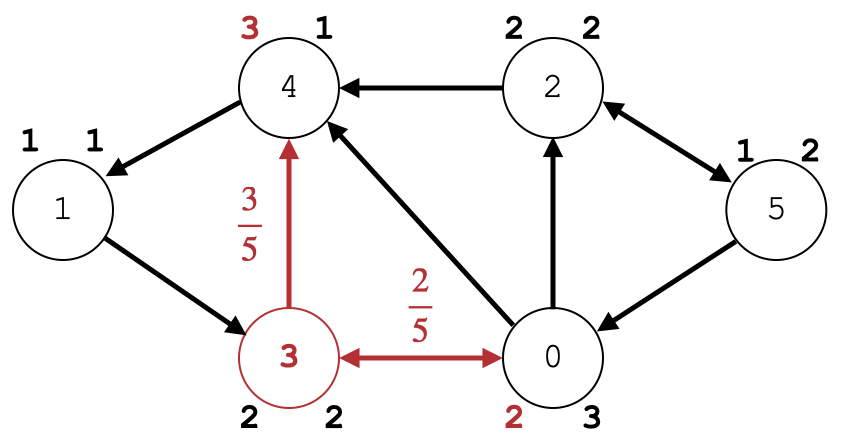
\includegraphics[scale=0.2]{3.png}\end{center}
\caption{The in-weight of edge (3,4) and edge (3,0).}
\end{figure}
\subsection{Out-Weight}
The out-weight of an edge is the ratio of the outdegree of \emph{dst} to the sum of the outdegrees of all nodes that \emph{src} cites as shown in Equation 2. The process for calculating the out-weight of an edge is very similar to the in-weight. Figure 4 shows how to calculate the out-weight for edge (3,4) and edge (3,0).
\begin{equation}
\large W^{out}_{(src,dst)}=\frac{outdegree_{dst}}{\sum_{k\in out(src)}outdegree_{k}}
\end{equation}
The in-weight and out-weight for every edge is shown in Figure 5. This diagram will be a good reference for calculating the weighted page rank algorithm in the next section.
\begin{figure}[h!]
\begin{center}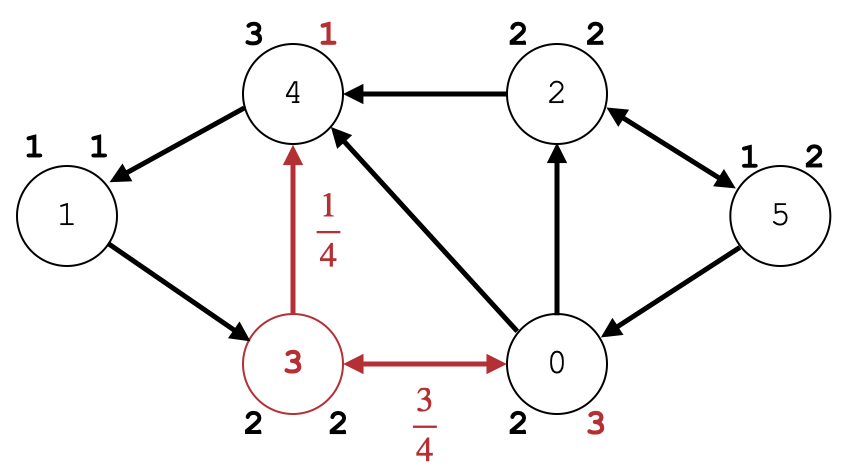
\includegraphics[scale=0.2]{4.png}\end{center}
\caption{The out-weight of edge (3,4) and edge (3,0).}
\end{figure}
\begin{figure}[h!]
\begin{center}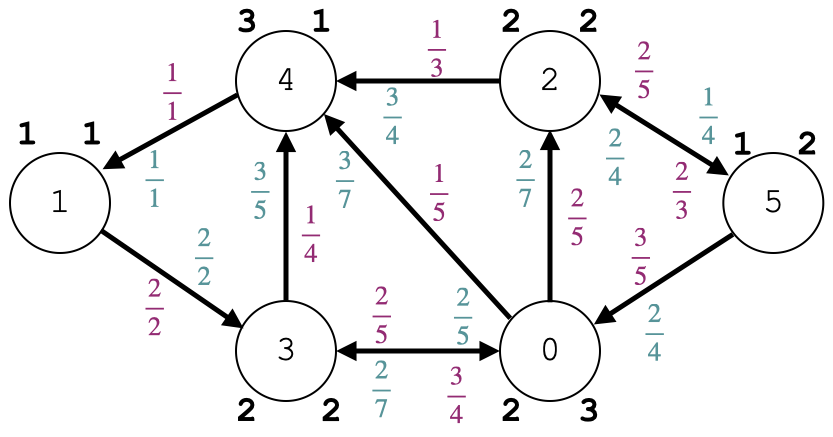
\includegraphics[scale=0.2]{5.png}\end{center}
\caption{The in-weight (blue) and out-weight (purple) for every edge.}
\end{figure}
\subsection{Weighted Page Rank Algorithm}
The page rank of an article is exactly as it sounds--the articles with higher ranks are more popular and thus hold more weight \cite{weighted}. Here we calculate the page ranks of all 6 articles given Equation 3.
\begin{equation}
PR(dst)= \frac{1-d}{N}+d\sum_{v\in in(dst)}{PR(src)*W^{in}_{(src,dst)}*W^{out}_{(src,dst)}}
\end{equation}
First, we initialize the variables. The constant \emph{d} = 0.85, the number of articles \emph{N} = 6, and the initial page rank $PR(src)=PR(dst)=\frac{1}{N}=\frac{1}{6}$.\\\\
Second, for every \emph{dst}, we find the product of the in-weight and out-weight from Figure 5 and the page rank of \emph{src}. For example, the sum for node 4 is shown in Equation 4.
\begin{eqnarray*}
\sum_{v\in in(4)}{PR(src)*W^{in}_{(src,4)}*W^{out}_{(src,4)}}\\
\end{eqnarray*}
\begin{equation}
=\frac{1}{6}*\frac{3}{5}*\frac{1}{4}+\frac{1}{6}*\frac{3}{7}*\frac{1}{5}+\frac{1}{6}*\frac{3}{4}*\frac{1}{3}=0.08095
\end{equation}
Third, calculate the remainder of the page rank equation for node 4.
\begin{equation}
PR(4)=\frac{1-0.85}{6}+0.85(0.08095)=0.09381
\end{equation}
\subsection{Iterative Page Rank}
The page rank was calculated for every \emph{dst}. This process was run 10 times. Every iteration inserted the updated $PR(src)$ and generated a new page rank for \emph{dst}. The final page ranks are shown in Figure 6.\\\\
After 10 iterations, the highest ranked node is 3 at 0.086. Node 1 is the next with 0.066 which may be surprising as it only has 1 indegree and 1 outdegree. However, its only indegree stems from node 4 which has the highest indegree in the graph. If article 4 is popular, then the only article it references must also be significant.\\
\begin{figure}[h!]
\begin{center}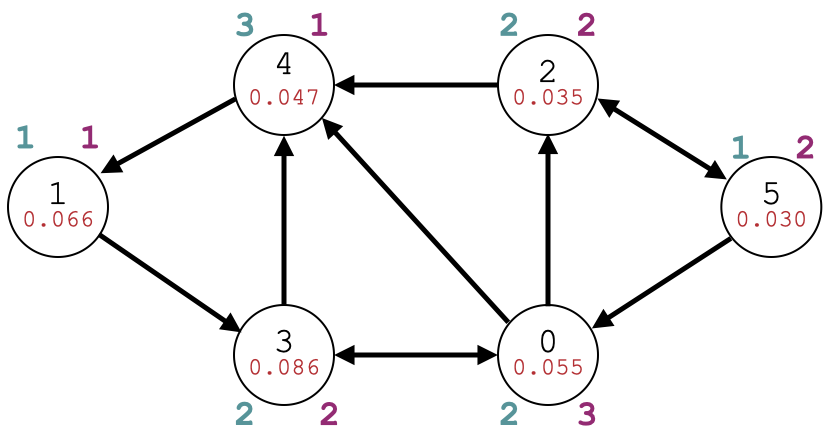
\includegraphics[scale=0.2]{6.png}\end{center}
\caption{The page ranks (red) after 10 iterations for each \emph{dst}.}
\end{figure}
\subsection{Clustering Coefficient}
The clustering coefficient is a measure of centrality \cite{cluster}. A node with a high coefficient (closer to 1) indicates that more of its neighbors are connected. Equation 6 is the clustering coefficient formula for a node where $t_{v}$ is the number of triangles that \emph{v} is a part of and $k_{v}$ is the number of degrees $(indegrees+outdegrees)$ of \emph{v}.\\\\
Note, to avoid dividing by 0, $k_{v}$ must be greater than 1. Therefore, nodes with less than 2 degrees should be filtered out. In this sample dataset, all nodes have at least 2 degrees.\\\\
\begin{equation}
CC(v)=\frac{2t_{v}}{k_{v}(k_{v}-1)}
\end{equation}\\\\
A triangle is a set of 3 nodes that form a \emph{clique} where one can traverse all edges and return to the original node. Figure 7 shows the 2 triangles that node 3 is a part of. The degrees and triangles for every node is listed in the table below along with its clustering coefficient.\\\\
\begin{figure}[h!]
\begin{center}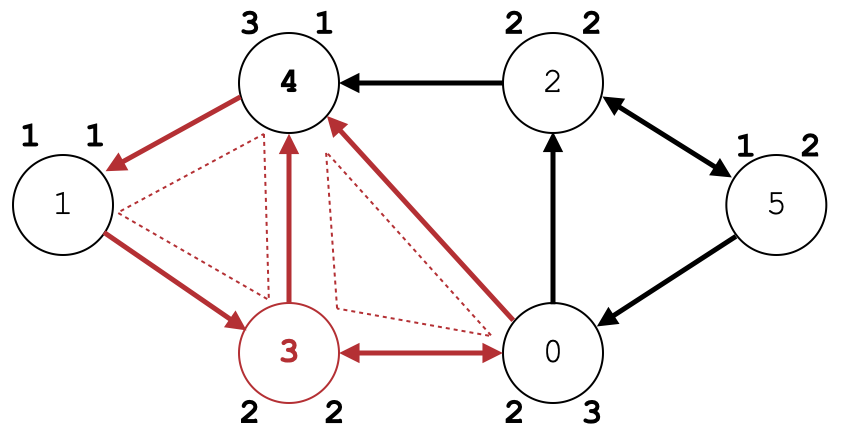
\includegraphics[scale=0.2]{7.png}\end{center}
\caption{The 2 triangles that node 3 is a part of.}
\end{figure}
\begin{center}
\begin{tabular}{ c c c c }
$v$ & $k_{v}$ & $t_{v}$ & $CC_{v}$\\ \hline
0 & 5 & 3 & 0.3\\
1 & 2 & 1 & 1.0\\
2 & 4 & 2 & 0.33\\
3 & 4 & 2 & 0.33\\
4 & 4 & 3 & 0.5\\
5 & 3 & 1 & 0.33\\
\end{tabular}
\end{center}
The clustering result of this small dataset is clearly visible in Figure 7. There is a moderate to high clustering coefficient for the articles in this dataset. Most are a part of 1 out of 3 possible triangles. The node with the highest proportion of cliques is node 1 which is connected to 2 other nodes and they are also connected.
\begin{thebibliography}{6}
\bibitem{acm} “About the ACM Organization.” Association for Computing Machinery, ACM, www.acm.org/about-acm/about-the-acm-organization.\\

\bibitem{tang} Jie Tang, Jing Zhang, Limin Yao, Juanzi Li, Li Zhang, and Zhong Su. ArnetMiner: Extraction and Mining of Academic Social Networks. In Proceedings of the Fourteenth ACM SIGKDD International Conference on Knowledge Discovery and Data Mining (SIGKDD'2008). pp.990-998.\\

\bibitem{sparksql} “Spark SQL, DataFrames and Datasets Guide.” Spark 2.4.5 Documentation, Apache, spark.apache.org/docs/latest/sql-programming-guide.html.\\

\bibitem{graphx} “GraphX Programming Guide.” GraphX - Spark 2.4.5 Documentation, Apache, spark.apache.org/docs/latest/graphx-programming-guide.html.\\

\bibitem{weighted} W. Xing and A. Ghorbani, "Weighted PageRank algorithm," Communication Networks and Services Research, 2004. Proceedings. Second Annual Conference on, 2004, pp. 305-314.\\

\bibitem{cluster} “05 Clustering Coefficient.” 05 Clustering Coefficient, Find Xrci, www.youtube.com/watch?v=K2WF4pT5pFY.\\
\end{thebibliography}

\end{document}